\documentclass[preview=true]{standalone}
\usepackage{pgfplots}
\pgfplotsset{compat=1.18}
\usepackage[utf8]{inputenc}
\usepackage{newtxtext,newtxmath}
\usepackage[T1]{fontenc}

\begin{document}
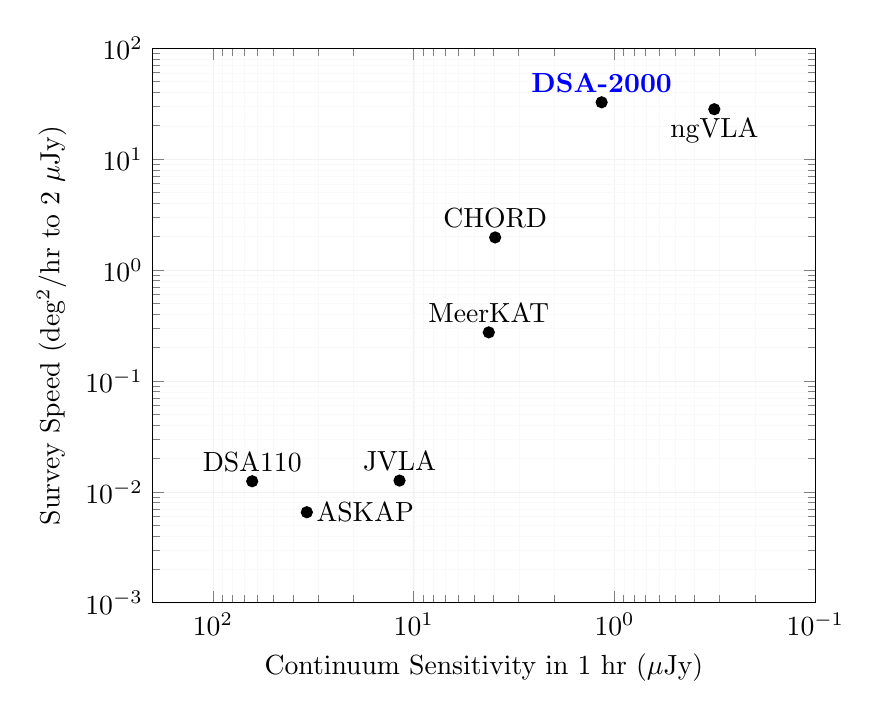
\begin{tikzpicture}
\begin{axis}[
    width=10cm,
    xlabel={Continuum Sensitivity in 1 hr ($\mu$Jy)}, 
    ylabel={Survey Speed (deg$^2$/hr to 2 $\mu$Jy)},
    ymode=log,
    xmode=log,
    grid={both},
    grid style={line width={.1pt},
    draw={gray!5}},
    major grid style={line width={.2pt},
    draw={gray!10}},
    x dir=reverse,
    xmin=0.1,
    xmax=200,
    ymin=0.001,
    ymax=100,
]

\addplot[scatter,
        nodes near coords,
        only marks,
        point meta=explicit symbolic,
        coordinate style/.from=\thisrow{style}
    ]
    table[meta=label] {
        x       y         label                 style
        1.16     32.51    {\textbf{DSA-2000}}   {above, blue}
        4.23     0.274    {MeerKAT}             above
        3.933    1.966    {CHORD}               above
        0.3186   28.149   {ngVLA}               below
        34.080   0.00655  {ASKAP}               {below, right}
        63.7627  0.01246  {DSA110}              above
        11.7744  0.01263  {JVLA}                above
    };
    
\end{axis}
\end{tikzpicture}
\end{document}